\documentclass{article}
\usepackage{amsfonts, amsthm, amsmath}

\usepackage{geometry, graphicx}
\usepackage{algorithm, algorithmic}
\usepackage{bm}
\geometry{left = 5em, right = 5em}

\def\showtopic{Mathematical Image Processing Homework 3}
\def\showtitle{Level Set Method}
\def\showabs{Level Set Method}
\def\showauthor{Yuanfeng Shi, 1800010697}

\title{\showtitle}
\author{\showauthor}

\usepackage{fancyhdr}  
\pagestyle{fancy}
\lhead{\textbf {\showtopic} }
\chead{} 
\rhead{\textbf {\showabs} }
\lfoot{} 
\cfoot{\thepage}
\rfoot{} 
\renewcommand{\headrulewidth}{0.4pt} 


\usepackage{listings}
\lstset{language=Matlab}
\lstset{breaklines}
\lstset{extendedchars=false}
\newtheorem{remark}{Remark}
\begin{document}
\maketitle
\thispagestyle{fancy}
\section{Level Set Method}
Let us first take a look at the curve evolution equations:

$$\left\{ \begin{array} { l } { \frac { \partial c } { \partial t } = F N } \\ { c ( 0 , q ) = c _ { 0 } ( q ) } \end{array} \right.$$
A key observation is that a curve $c$ can be seen as the zero level set of some function $u$ in higher dimension:
$$u ( t , c ( t , q ) ) = 0,$$
$$\frac { \partial u } { \partial t } + \left\langle \nabla u , \frac { \partial c } { \partial t } \right\rangle = \frac { \partial u } { \partial t } + \langle \nabla u , F N \rangle = 0.$$
$$\frac { \partial u } { \partial t } ( t , c ( t , q ) ) = F | \nabla u ( t , c ( t , q ) ) |.$$
\section{Active Contour}

The active contour method aims to minimize the energy of the curve:
$$J(c) = \int g(|\nabla I(c(q))|) |c'(q)| dq.$$
First we take a look at the flow of the Geodestic active cintours model:
$$\frac{\partial c}{\partial t} = (\kappa g - \langle\nabla g,N \rangle )N.$$
Here $\kappa$ is the curvature of the curve. 
The drawback of the original model is that it is hard to detect nonconvex objects. In order to let the curve cling to the edge, we propose an improved equation to plug the contour into the nonconvex region:
$$
\frac{\partial c}{\partial t} = (\kappa g - \langle\nabla g,N \rangle  + \alpha g)N.$$

We solve this method using level set method, suppose $u$ is the level set function, then we induce the evolution equation of the $u$:

\begin{equation}
\label{model:ac}
\frac{\partial u}{\partial t} = g(|\nabla I|)\left(div \left(\frac{\nabla u}{|\nabla u|}\right) + \alpha\right) |\nabla u| + \langle \nabla g, \nabla u\rangle.\end{equation}

\section{Convexified CV}
\subsection{Model}
We list our energy model, which is slight different from the formula in the SLIDE (the limit of $u$):
$$\min_{|u|\le 1}\int_D |\nabla u| + \lambda \int_D \{(c_1-f(x))^2 - (c_2-f(x)^2\}u(x).$$
\subsection{Algorithm}

We set $\bm{d} = \nabla u$ and use the augmented Lagrangian method to solve the constrained problem:
$$\min_{\bm{d},u\in[-1,1]} \|\bm{d}\|_1 + \mu\langle u,r \rangle~~~~s.t. ~~ \bm{d} = \nabla u.$$
We obtain the following algorithm:
$$\left\{ \begin{array}{rl} (u^{k+1}, \bm{d}^{k+1}) & = argmin_{u\in [-1,1], \bm{d}} \|\bm{d}\|_1 + \mu\langle u,r \rangle + \frac{\lambda}{2} \|\bm{d} - \nabla u - \bm{b}^k\|_2^2\\ \bm{b}^{k+1} &= \bm{b}^k + \delta(\nabla u - \bm{d}^k) \end{array} \right.$$

We alternatively optimize the $u$ and $\bm{d}$. In order to avoid the near singularity of $\nabla^T \nabla$ when solving it using FFT, we consider replace $\nabla^T \nabla$ by $\nabla^T \nabla + \epsilon I$, where $I$ is the identity operator.
 
The whole algorithm is shown in Algorithm

\begin{algorithm}[H]
\caption{$u = ms(f,lambda,outer iter, inner iter)$}
\begin{algorithmic}
\STATE Initialize the level set function $u$.
\FOR {$i$=1:outer iter/inner iter}
\STATE Update two area $u>0$ and $c<0$.
\STATE Calculate the mean value of $f$ in two area: $c_1$, $c_2$.
\FOR {$j$ = 1:inner iter}
\STATE $u = (\Delta^T\Delta + \epsilon I)^{-1}(\Delta^T(\bm{b}-\bm{d}) - \mu r)$
\STATE $\bm{d} = \mathcal{T}_{1/\lambda}(\bm{d})$

\STATE $\bm{b} = \bm{b} + \delta(\nabla u - \bm{d})$
\ENDFOR
\ENDFOR

\end{algorithmic}

\end{algorithm}

\section{Numerical Aspect}
\subsection{Result: Active contour}
We first show the result of the active contour method.  All the experiment uses the same initialization method and share the same reinforce iteration time 20. 

First we discuss the different choice of $$g(s) = \frac{1}{1+k|s|^2},$$
where $k$ is the only parameter to control the stiffness of $g$. Qualitatively, when $k$ is larger, the gradient is small hence negligible in the whole image. Thus the active contour method will fill in the sense all the level set function will be positive eventually, and in consequence the zero level set vanishes. When $k$ is small, the evolution will be stuck at some smooth area and thus fail. 

\begin{figure}[H]
\caption{The affects of the choice of $k$: k=0.1,0.01(optimal),0.005,0.001}
\begin{center}
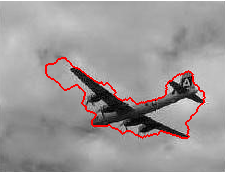
\includegraphics[scale=.7]{k1.png}
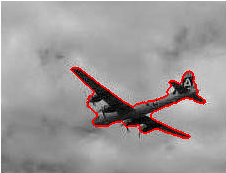
\includegraphics[scale=.7]{k01.png}
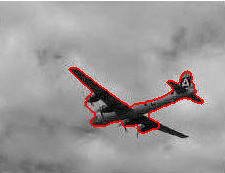
\includegraphics[scale=.7]{k005.png}
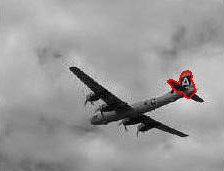
\includegraphics[scale=.7]{k001.png}
\end{center}
\end{figure}

Then we show the results of different iteration time.
\begin{figure}[H]
\caption{The result of the active contour: iter \_ time = 1000,2000,4000, $g(s) =\frac{1}{1+0.01s^2}$}
\begin{center}
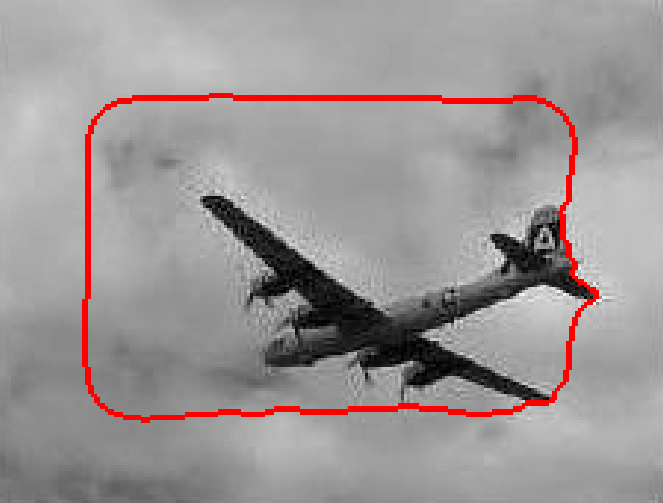
\includegraphics[scale=.28]{iter1000.png}
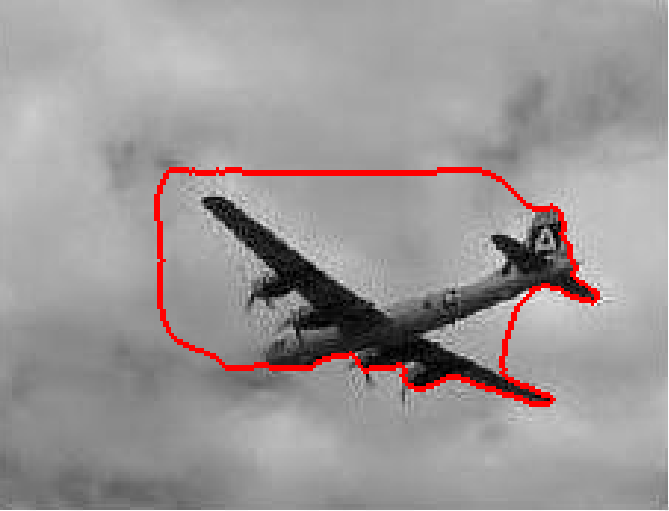
\includegraphics[scale=.27]{iter2000.png}
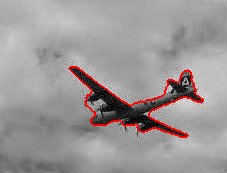
\includegraphics[scale=.81]{iter4000.png}
\end{center}
\end{figure}
The effects of noise and blurring: When the noise size become larger, the $g$ is supposed to chose more stiff to make the evolution faster.
\begin{figure}[H]
\begin{center}
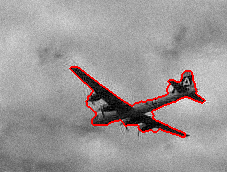
\includegraphics[scale=.8]{sigma03.png}
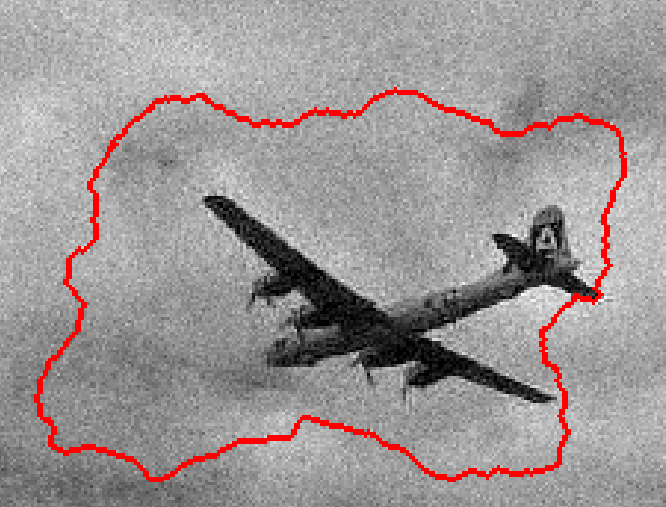
\includegraphics[scale=.27]{sigma05.png}
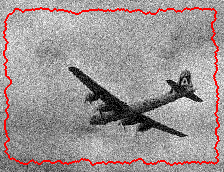
\includegraphics[scale=.8]{sigma1.png}
\caption{Different Gaussian white noise size affects the segmentation result. Noise size = 0.03, 0.05, 0.1.}
\end{center}
\end{figure}

\begin{figure}[H]
\caption{Different blur kernel size affects the segmentation result. Sigma = 0.5, 1, 2. Kernel\_size = 15}
\begin{center}
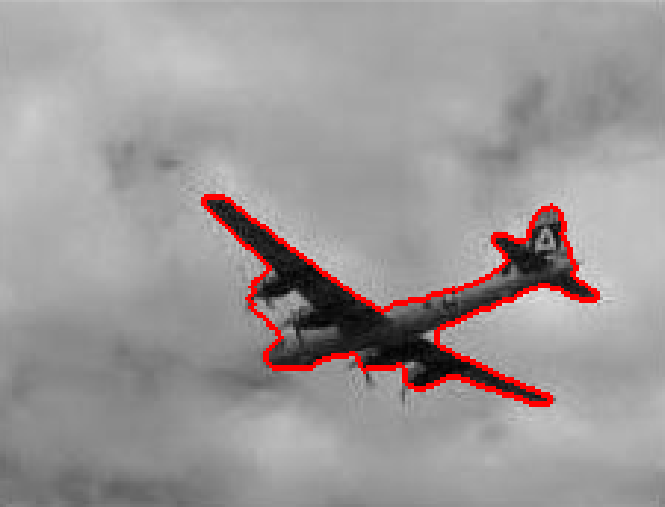
\includegraphics[scale=.3]{blur05.png}
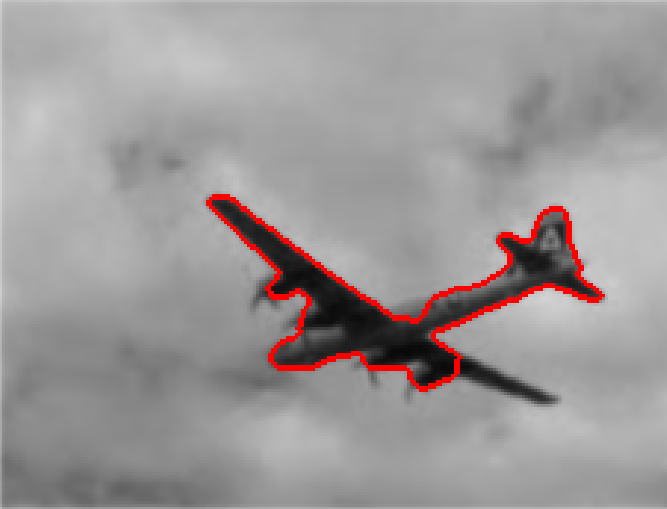
\includegraphics[scale=.3]{blur1.png}
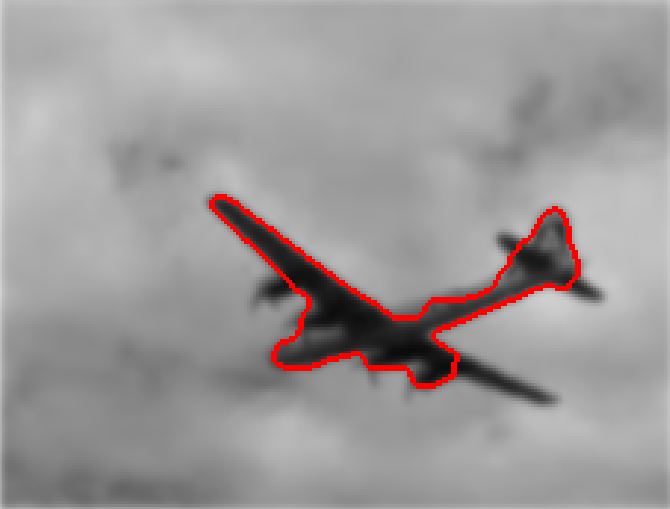
\includegraphics[scale=.3]{blur2.png}
\end{center}
\end{figure}

At last we show some other excellent results. 

\begin{figure}[H]
\begin{center}
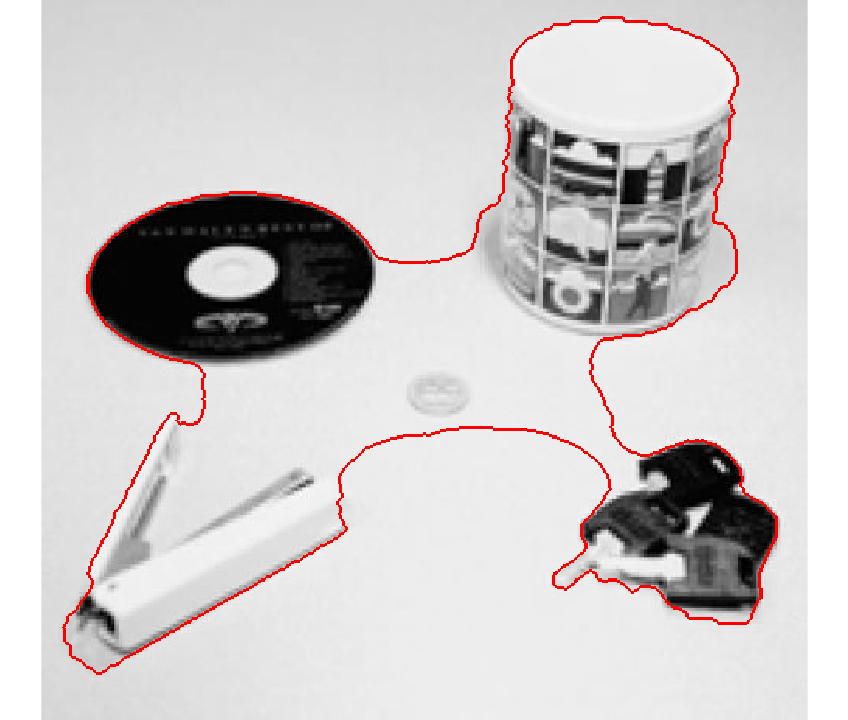
\includegraphics[scale=.47]{ac_1.png}
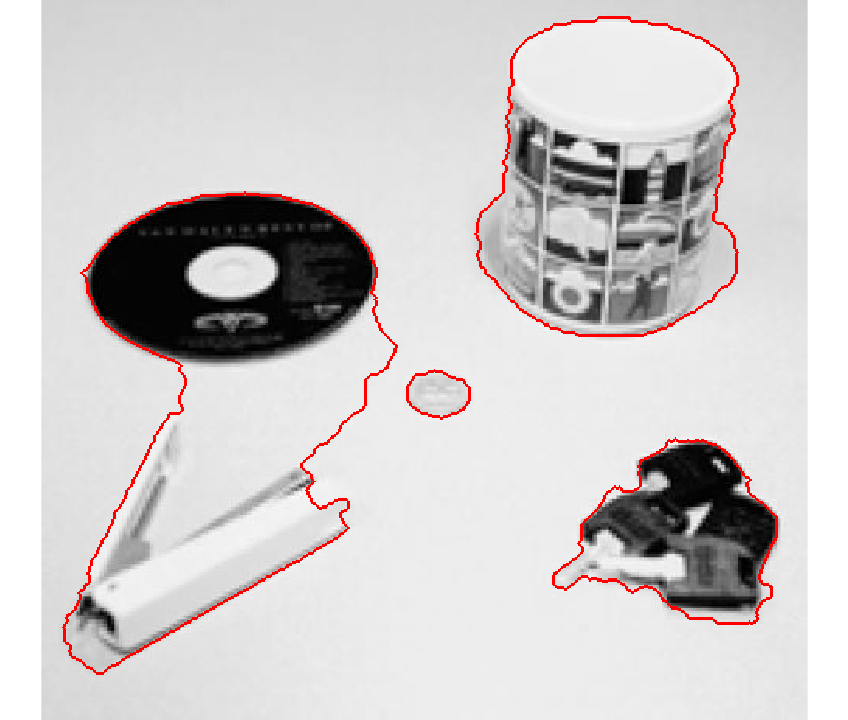
\includegraphics[scale=.47]{ac_4.png}
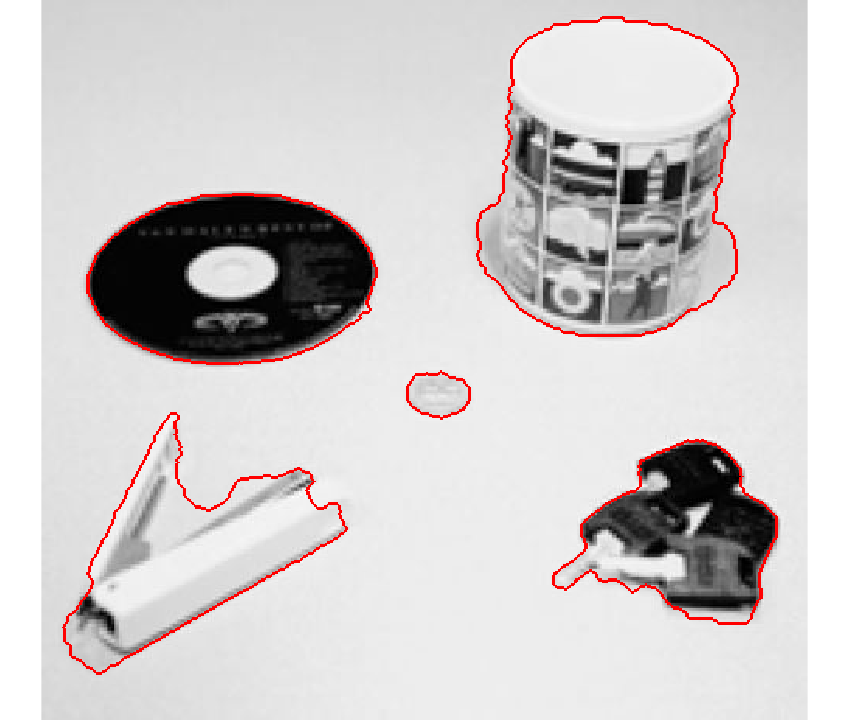
\includegraphics[scale=.47]{ac_2.png}
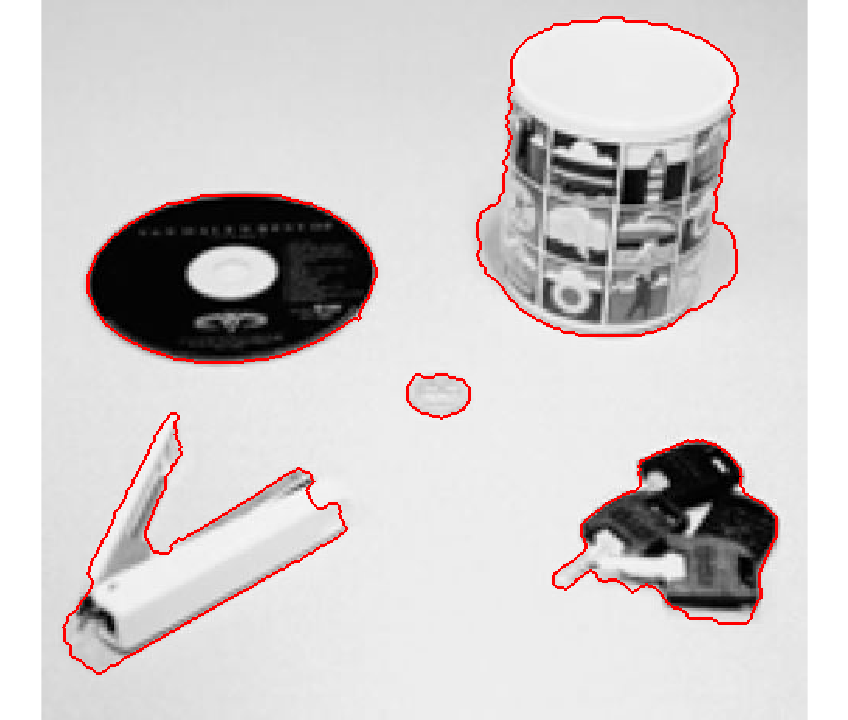
\includegraphics[scale=.47]{ac_3.png}
\end{center}
\caption{The result of the active contour: iter\_ time = 8000,12000,16000,20000, $g(s) =\frac{1}{1+0.5s^2}$}
\end{figure}

\subsection{Result: Convexified CV model}

Now we focus on the result of the relaxed MS model. For simplicity, all the experiment uses the same initialization method and share the same inner iteration time 20. We first observe that Convexified CV model take shorter iteration time to stop. 

\begin{figure}[H]
\caption{The result of the active contour: iter \_ time = 1,5,20,100}
\begin{center}
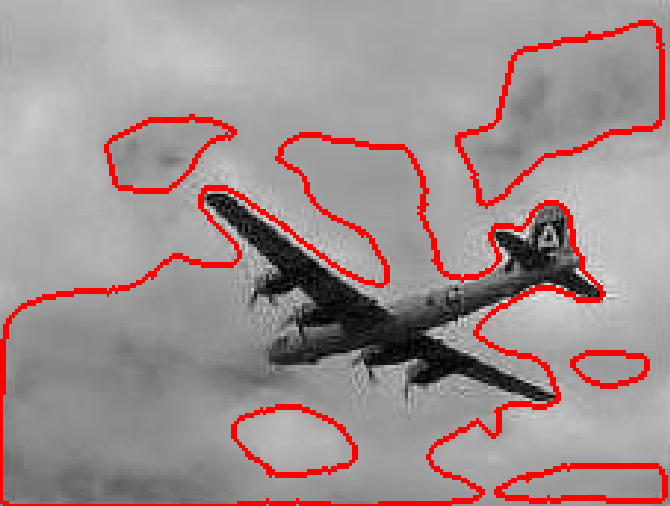
\includegraphics[scale=.23]{cv1.png}
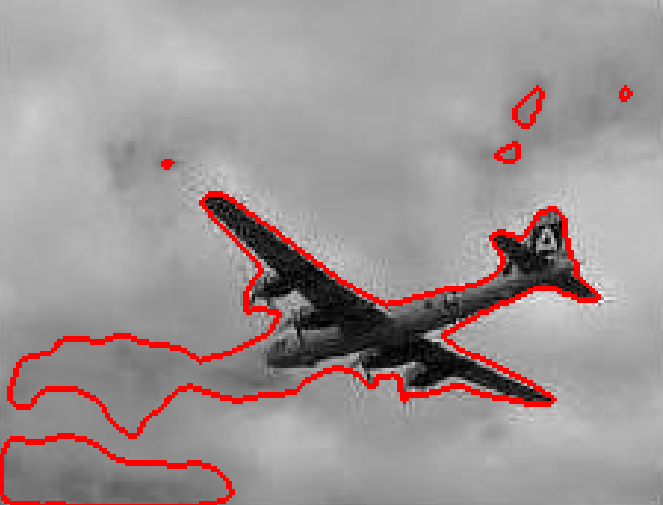
\includegraphics[scale=.23]{cv5.png}
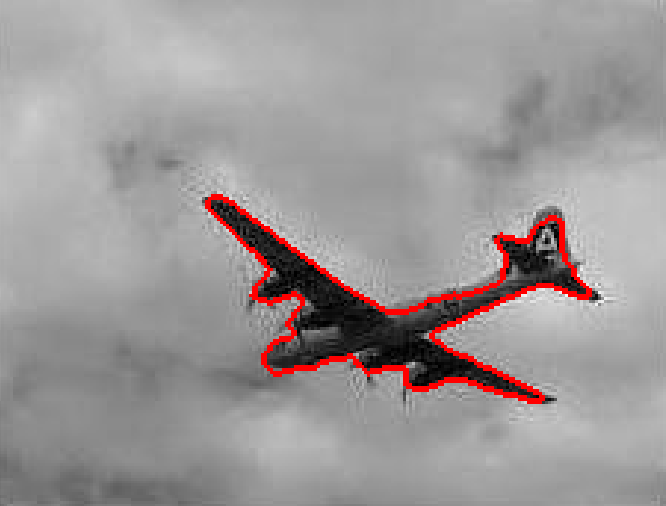
\includegraphics[scale=.23]{cv20.png}
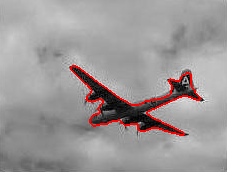
\includegraphics[scale=.68]{cv100.png}
\end{center}
\end{figure}

Besides, CV model show more robustness under different noise and blur settings. For Gaussian white noise, we implement it by ``noise\_size * randn(size(f))''. For blurring, we use ``fspecial('gaussian', 15, sigma)'' as our blur kernel.

\begin{figure}[H]
\caption{Different Gaussian white noise size affects the segmentation result. Noise size = 0.05, 0.1, 0.2.}
\begin{center}
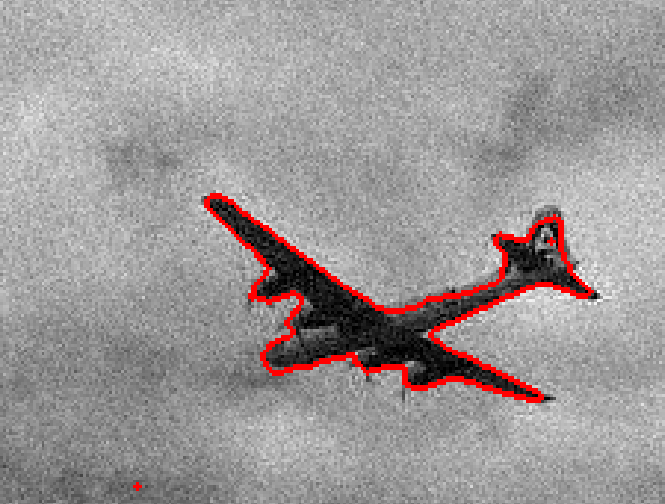
\includegraphics[scale=.27]{cv_sigma05.png}
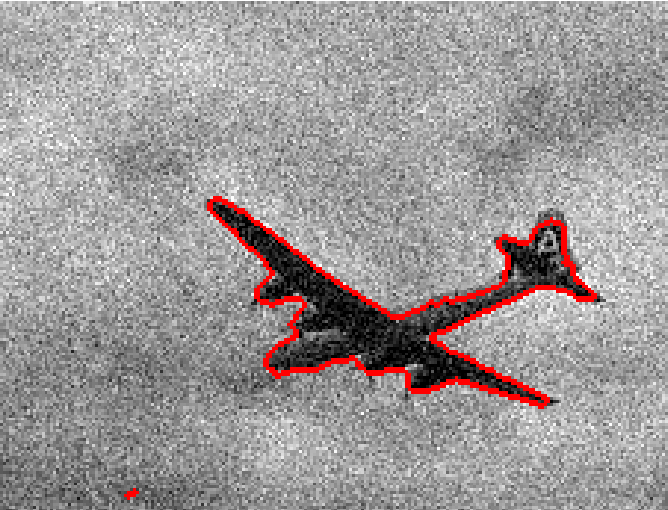
\includegraphics[scale=.27]{cv_sigma1.png}
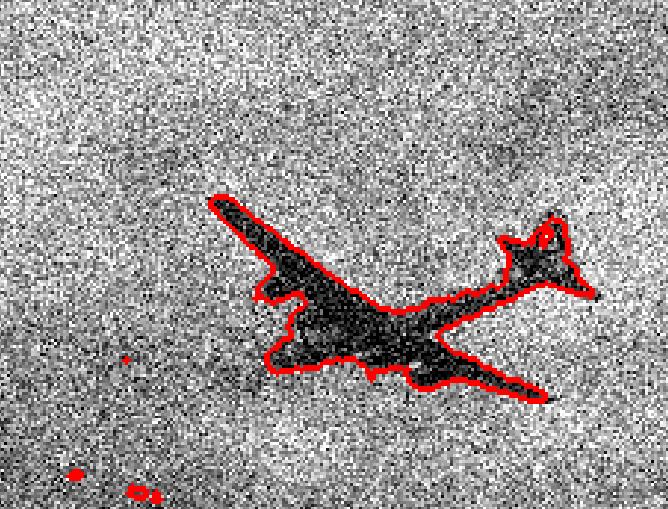
\includegraphics[scale=.27]{cv_sigma2.png}
\end{center}
\end{figure}

\begin{figure}[H]
\caption{Different blur kernel size affects the segmentation result. Sigma = 0.5, 1, 2.}
\begin{center}
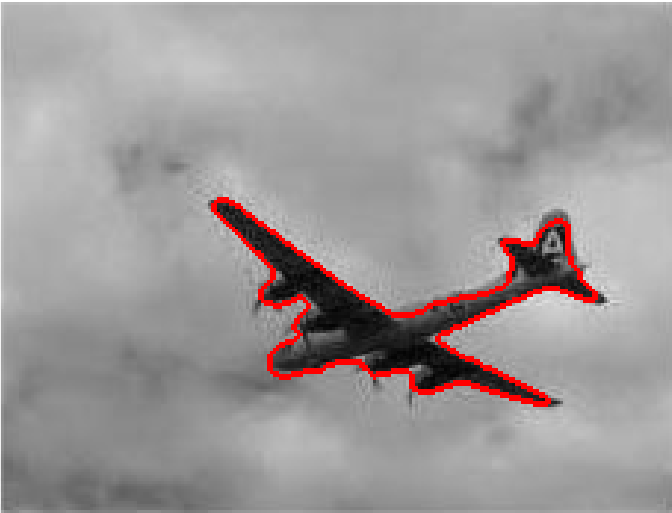
\includegraphics[scale=.27]{cv_blur05.png}
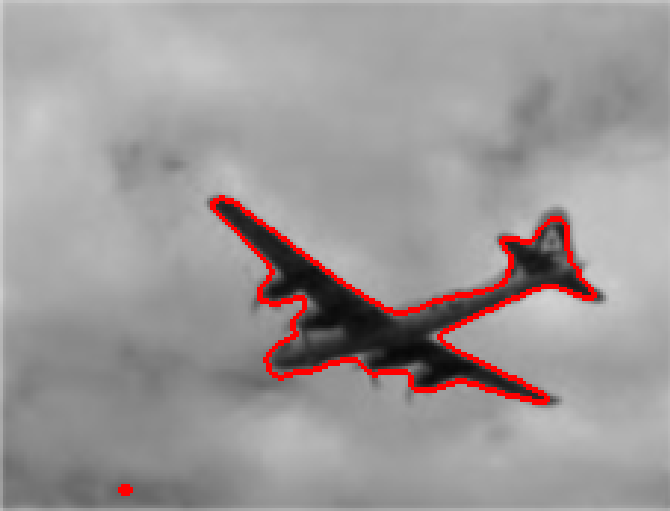
\includegraphics[scale=.27]{cv_blur1.png}
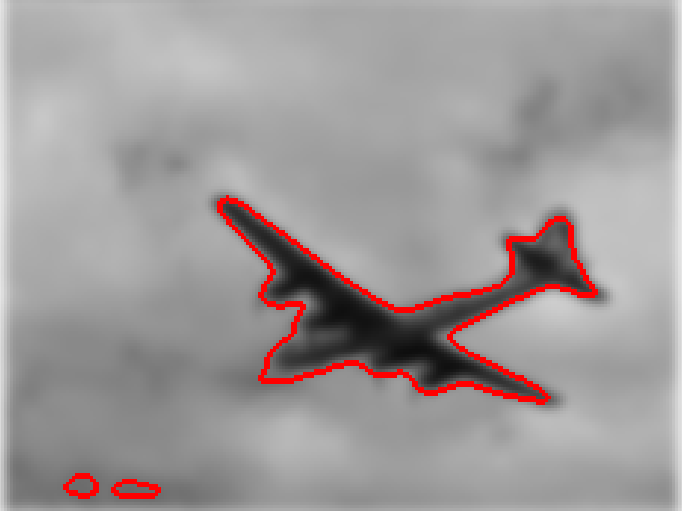
\includegraphics[scale=.27]{cv_blur2.png}
\end{center}
\end{figure}

However, this method will fail to obtain the true result in some pictures.
\begin{figure}
\begin{center}
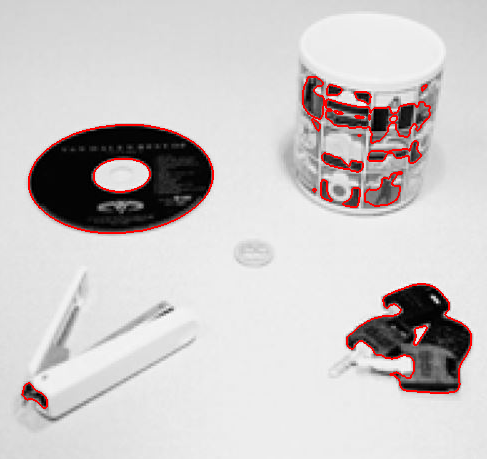
\includegraphics[scale=.5]{failure.png}
\end{center}
\end{figure}

We conclude that CV model cannot deal with object segmentation when the diversity of color in objects is high.

\end{document}



